\subsection{Espectroscopia Mössbauer}

\begin{figure}[h!]
    \centering
    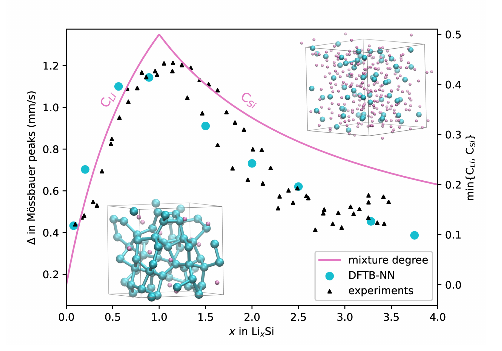
\includegraphics[width=.7\textwidth]{Silicio/prediccion/resultados/mossbauer/mossbauer.png}
    \caption{Desplazamiento entre los dos picos en los espectros de efecto 
    Mössbauer. Los triángulos que apuntan hacia arriba corresponden a dos 
    medidas de Li \text{et al.} (eje de la izquierda), la línea continua es la 
    predicción de la ecuación \ref{eq:mossbauer}, utilizando concentraciones 
    medias de átomos de Li y Si. Los círculos azules son las predicciones dada 
    por la ecuación \ref{eq:mossbauer}, con $C_{\text{Li}}$ , $C_{\text{Si}}$ 
    calculados a partir de la concentración de los vecinos más cercanos (eje de 
    la derecha). Las barras de error son menores que el tamaño de los puntos.}
    \label{fig:mossbauer}
\end{figure}
